\section{CSA für OTP}

\subsection{Datenstruktur}
Der CSA benötigt zwei Datenstrukturen. Eine Zeittafel (TimeTable) für die Eingabe von Daten und eine Reise (\texttt{Journey}) für die Rückgabe von Daten. 

\subsubsection{Zeittafel (\texttt{TimeTable})}
Der \texttt{TimeTable} ist eine \hypertarget{timetable}{Zeittafel}, die alle benötigen Daten für den CSA zur Verfügung stellt. Die Datenstruktur ist ein Quadrupel aus Sammlungen von Fusswegen (\texttt{FootpathCSA}), Haltestellen (\texttt{StopCSA}), Verbindungen (\texttt{ConnectionCSA}) und Fahrten (\texttt{TripCSA}).\newline 
Neben den \texttt{.add()}- und \texttt{.show()}-Funktionen für die Sammlungen enthält die \texttt{TimeTable}-Klasse die Methode \texttt{.getFootpathChange()}, welche für eine Haltestelle die Umsteigzeit zurückgibt.

\begin{figure}[htb]
	\centering
	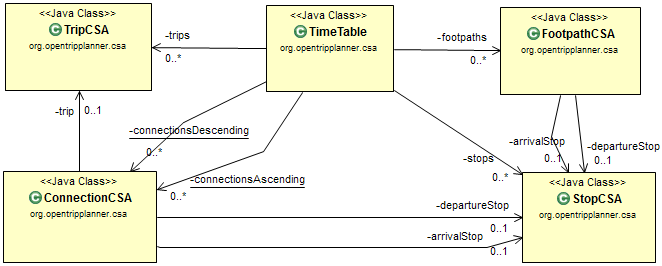
\includegraphics[width=8cm]{img/TimeTable.png}
	\caption{UML-Diagramm zu \texttt{TimeTable}-Datenstruktur.}
	\label{fig:uml-timetable}
\end{figure}

\subsubsection{Fusswege (\texttt{FootpathCSA})}

Ein \hypertarget{footpath}{Fussweg} kann zwei verschiedene Funktionen haben. Er besteht aus einem DepartureStop, einem ArrivalStop sowie einer Dauer. Wenn der DepartureStop und der ArrivalStop gleich sind, repräsentiert der Footpath einen Umsteigeprozess. Wenn sie unterschiedlich sind, repräsentiert er einen Laufweg zu einem Stop hin oder von einem Stop weg.

\begin{figure}[htb]
	\centering
	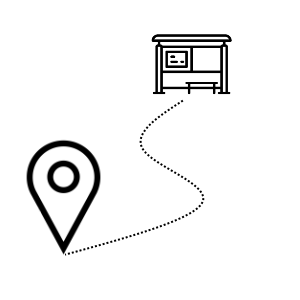
\includegraphics[width=5cm]{img/footpath.png}
	\caption{Symbolbild für den Fussweg (FootpathCSA).}
	\label{fig:footpath}
\end{figure}


\subsubsection{Haltestellen (\texttt{StopCSA})}

Ein Stop ist eine \hypertarget{stop}{Haltestelle} für öffentliche Verkehrsmittel. Ein Stop besitzt einen Namen, Längen- und Breitengrad. 

\begin{figure}[htb]
	\centering
	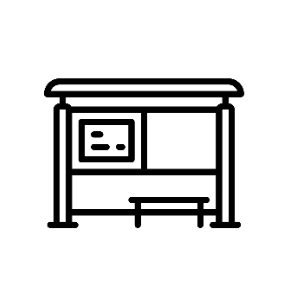
\includegraphics[width=5cm]{img/stop.png}
	\caption{Symbolbild für die Haltestelle (StopCSA)\cite{stop-pic}}
	\label{fig:stop}
\end{figure}

\subsubsection{Verbindungen (\texttt{ConnectionCSA})}

Eine Connection ist eine \hypertarget{connection}{Verbindung} zwischen einem DepartureStop und einem ArrivalStop . Die Connection hält Daten fest wie die Abfahrtszeit vom DepartureStop und die Ankunftszeit vom ArrivalStop. Zudem weiss die Connection zu welchem Trip sie gehört.

\begin{figure}[htb]
	\centering
	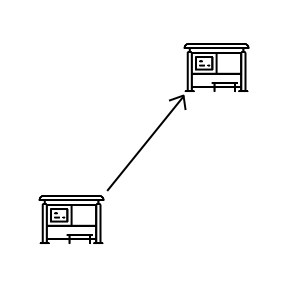
\includegraphics[width=5cm]{img/connection.png}
	\caption{Symbolbild für die Verbindung (ConnectionCSA)}
	\label{fig:connection}
\end{figure} 

\subsubsection{Fahrten (\texttt{TripCSA})}

Als Trip wird die \hypertarget{trip}{Fahrt} eines öffentlichen Verkehrsmittels von der Start-Station bis zur End-Station bezeichnet. Es ermöglicht den CSA, ohne Umsteigen erreichbare Orte zu erkennen. Ein Trip besteht aus mehreren Connections, die aneinandergereiht sind. Des weiteren hält der Trip Informationen über das Verkehrsmittel (Zug,Bus usw.) und welche Geschäftsorganisation dieses Verkehrsmittel zur Verfügung stellt. Ausserdem enthält der Trip Informationen, ob der Trip an jenem Tag auch stattfinden kann oder nicht.

\begin{figure}[htb]
	\centering
	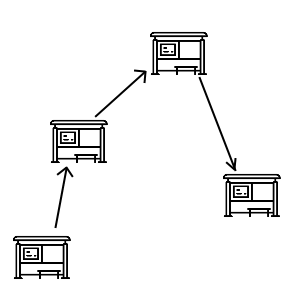
\includegraphics[width=5cm]{img/trip.png}
	\caption{Symbolbild für die Fahrt (TripCSA)}
	\label{fig:trip}
\end{figure}

\subsubsection{Reise (\texttt{Journey})}
Ein \hypertarget{journey}{Journey} ist ein vom CSA berechneter Weg vom Start- zum Zielpunkt. Er besteht aus einem StartPath, welcher den Fussweg zur ersten Station hin darstellt, sowie eine Liste aus JourneyPointer, welche den Weg mit allen Umsteigestationen repräsentiert.
 
\begin{figure}[htb]
	\centering
	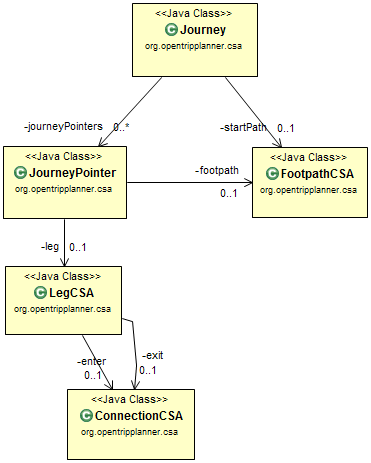
\includegraphics[width=8cm]{img/Journey.png}
	\caption{UML-Diagramm zur \texttt{Journey}-Datenstruktur im Überblick.}
	\label{fig:uml-journey}
\end{figure}

\subsubsection{Reisezeiger (\texttt{JourneyPointer})}
Ein \hypertarget{journeyPointer}{JourneyPointer} ist eine Hilfskonstruktion, welche der CSA anlegt, um die berechnete Abfolge von Stationen später wieder rekonstruieren zu können. Ein JourneyPointer besteht aus einem Leg sowie einem Footpath. Dabei handelt es sich beim Leg um eine Fahrt in einem ÖV vom Einsteigen bis zum Aussteigen und beim Footpath um das darauffolgende Umsteigen oder das Erreichen des Ziels.

\subsubsection{Fahrtabschnitte (\texttt{LegCSA})}
Ein \hypertarget{leg}{Leg} ist die Fahrt in einem öffentlichen Verkehrsmittel vom Einsteigen bis zum Aussteigen. Dies ermöglicht es, den Journey nicht von Station zu Station, sondern von Umsteigen zu Umsteigen zu rekonstruieren. Ein Leg besteht aus einer EnterConnection und einer ExitConnection. 

\subsection{Programmablauf}
\begin{figure}[htb]
	\centering
	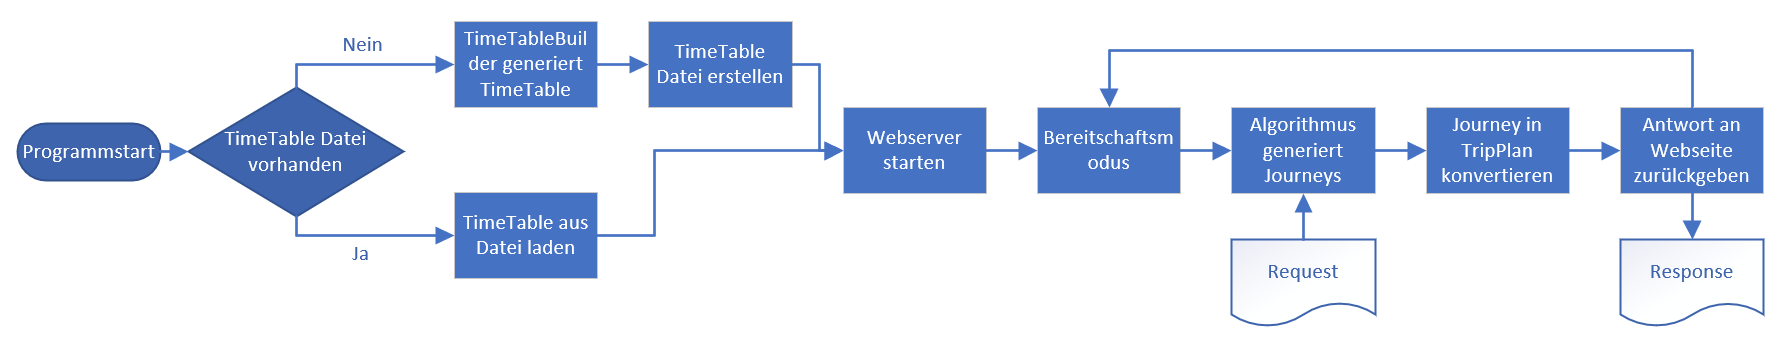
\includegraphics[width=15cm]{img/programmablauf.png}
	\caption{Programmablauf des OTP mit dem CSA.}
	\label{fig:programmablauf}
\end{figure}

\subsubsection{Zeittafelerzeuger (\texttt{TimeTableBuilder})}
Da wir für den CSA eine \hypertarget{timeTableBuilder}{Zeittafel} (\texttt{TimeTable}) benötigen, muss diese durch den Zeittafelerzeuger (\texttt{TimeTableBuilder}) erstellt werden. Die zugrundeliegenden \hyperlink{GTFS}{GTFS-Daten} können jedoch nicht in dieser Form einfach der Zeittafel übergeben werden. Der Zeittafelerzeuger erzeugt die Zeittafel. Durch die Funktion \texttt{.loadFromGtfs()} werden die Daten eingelesen und in die benötigte Form gebracht. Dieser Prozess kann durchaus einige Zeit in Anspruch nehmen. Deshalb wird, nachdem die Zeittafel fertig befüllt wurde, diese anschliessend serialisiert und als Java-SerializedObjectFile gespeichert. Somit brauchen wir nicht mehr jedesmal die Zeittafel komplett neu einzulesen und zu erstellen. Durch die Funktion \texttt{.loadFromSerializedObjectFile()} kann die zwischengespeicherte Zeittafel jederzeit eingelesen werden, was die Zeit, um eine schon in Form gebrachte Zeittafel zu erzeugen, um einiges verkürzt. Unabhängig von beiden Methoden wird dann der Server gestartet.

\subsubsection{Server}
Der Server wird über die Main-Funktion gestartet. Bei dem Server handelt es sich um einen \texttt{GrizzlyServer}. Der Server stellt eine Webseite zur Verfügung (Webserver). Über diese Webseite kommuniziert der Server mit allen Clients, indem er alle Requests (Anfragen) entgegen nimmt und alle dazugehörigen Responses (Antworten) zurückschickt. Die Kommunikation läuft hierbei über ein HTTP-Protokoll zwischen Server und Clients (Browser). 

\begin{figure}[htb]
	\centering
	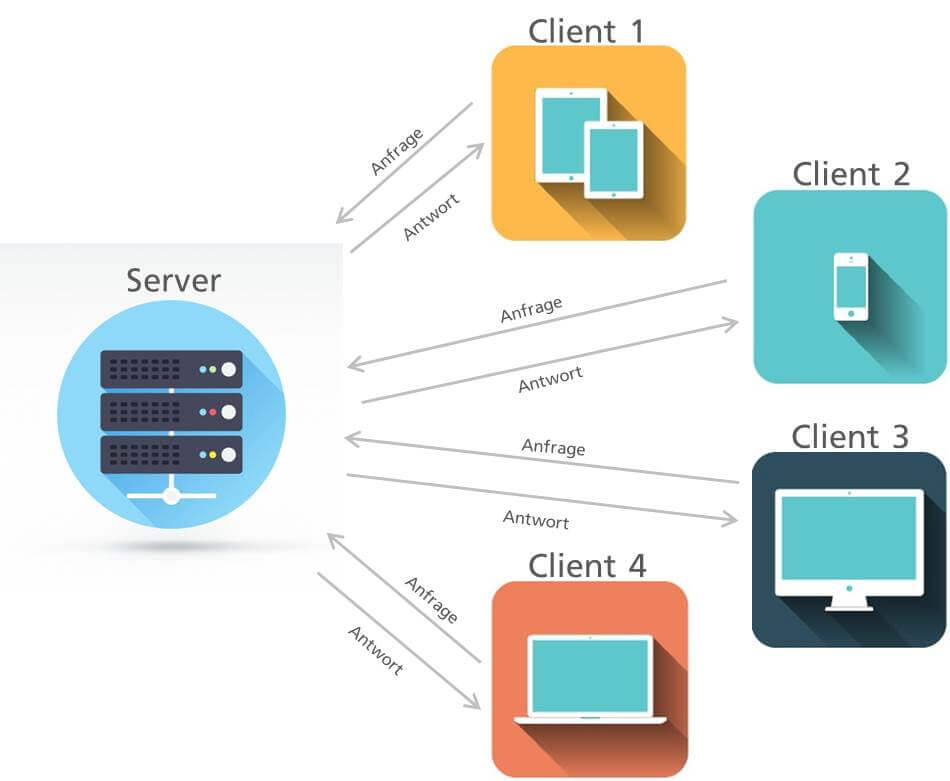
\includegraphics[width=8cm]{img/serverrequestresponse.jpg}
	\caption{Darstellung der Kommunikation zwischen Clients und Server\cite{server-pic}.}
	\label{fig:serverrequestresponse}
\end{figure}




\subsubsection{Webseitenaufruf}
Wenn ein Aufruf von der Webseite eingeht, so wird die \texttt{plan()}-Methode der Klasse PlannerResource aufgerufen. Diese erhält die Anfragenparameter in einem \texttt{RoutingRequest}-Objekt. Das im Preprocessing generierte TimeTable-Objekt wird als neue Instanz übergeben. Dies wird gemacht, da der OTP eine seperate Instanz des Algorithmus für jeden Aufruf verwendet. Der TimeTable sowie der Request werden dann der \texttt{createJourneys}-Methode des Algorithmuses übergeben. Dessen Rückgabe wird in einem Set von Journeys gespeichert.


\subsubsection{Earliest Arrival Connection Scan}
Der \hypertarget{EAS}{Earliest Arrival Connection Scan Algorithmus}\cite{csa}, kurz EACS, ist ein Wegfindungsalgorithmus, welcher ein \gls{MEAT} (Minimum Expected Arrival Time) Problem löst. Er sucht sich den schnellsten Weg vom Start zum Zielpunkt und beendet dann seine Suche, ohne nach Alternativen zu suchen. \newline

EACS arbeitet mit einer nach Abfahrtszeit sortierten Liste von Verbindungen. Über diese iteriert er dann aufsteigend, wobei als Startpunkt die erste Verbindung verwendet wird, welche nach der im Request spezifizierten Abfahrtszeit abfährt. \newline

Jede Verbindung wird auf drei Eigenschaften überprüft:
\begin{itemize}
	\item Ist der Abfahrtsort der Startort?
	\item Wurde der Abfahrtsort schon von einer früheren Verbindung erreicht?
	\item Wurde das zur Verbindung gehörende Fahrzeug schon von einer früheren Verbindung benutzt?
\end{itemize}

Wenn eine dieser drei Bedingungen erfüllt ist, so wird dies im Ankunftsort der Verbindung mit einem Zeiger auf dem Ort vermerkt, bei welchem man in das jeweilige öffentlichen Verkehrsmittel eingestiegen ist. Der Ort, bei welchem man eingestiegen ist, wird mithilfe eines \texttt{Trip-Bits} gespeichert. Wenn ein öffentliches Verkehrsmittel zum ersten Mal verwendet wird, so wird der Startort gespeichert und das \texttt{Trip-Bit} wird für das öffentliche Verkehrsmittel gesetzt. Wird das öffentliche Verkehrsmittel erneut verwendet, so ist das \texttt{Trip-Bit} bereits gesetzt und der Startort wird nicht überschrieben. \newline

Sobald der Algorithmus eine Verbindung findet, welche eine der drei Bedingungen erfüllt und gleichzeitig der Ankunftsort dem Zielort entspricht, hat er einen Journey zum Ziel gefunden. Die Schleife wird unterbrochen und der Algorithmus baut sich vom Zielort aus mithilfe der Zeiger den kompletten Journey, auf welcher dann als Antwort zurückgegeben wird. \newline

Alternativ kann der EACS auch nur die früheste Ankunftszeit anstelle des kompletten Journeys zurückgeben. In dieser Version müssen keine Zeiger gespeichert werden, was den Algorithmus schneller macht. Es gehen jedoch Informationen über den Reiseweg verloren.

\subsubsection{Profile Connection Scan}
Der \hypertarget{PCS}{Profile Connection Scan Algorithmus}\cite{csa}, kurz PCS, ist ein Wegfindungsalgorithmus, welcher alle möglichen Reisen in einem bestimmten Zeitraum errechnet und sich anschliessend nach den gewünschten Kriterien die  beste Reise zurückgibt. \newline

Er arbeitet auch mit einer nach Abfahrtszeiten sortierten Liste von Verbindungen. Im Gegensatz zum EACS iteriert er absteigend über die Verbindungen. Er sucht also die Verbindung vom Zielpunkt aus. Jede Verbindung durchläuft dabei drei Prüfungen:

\begin{itemize}
	\item Kommt man ans Ziel, wenn man aussteigt?	\newline
	Diese Bedingung überprüft, ob der Ankunftsort der Verbindung der Zielort des Requests ist. Ist dies der Fall, so wird im Abfahrtsort der Verbindung die Ankunftszeit sowie die dazugehörige Verbindung gespeichert. Zusätzlich wird die Ankunftszeit für das jeweilige öffentliche Verkehrsmittel gespeichert.
	\item Kommt man ans Ziel, wenn man umsteigt? \newline
	Es wird überprüft, ob vom Ankunftsort der Verbindung schon ein Weg gefunden wurde, welcher zum Zielort führt. Dazu wird überprüft, ob im Ankunftsort eine Ankunftszeit gespeichert wurde. Ist dies der Fall, so wurde schon ein möglicher Weg vom Ankunftsort zum Zielort gefunden. Dann werden die Informationen wie in der ersten Bedingung im Abfahrtsort und dem öffentlichen Verkehrsmittel gespeichert.
	\item Kommt man ans Ziel, wenn man sitzen bleibt? \newline
	Es wird überprüft, ob von diesem öffentlichen Verkehrsmittel aus schon ein Weg zum Zielort gefunden wurde. Dazu wird überprüft, ob für das öffentlichen Verkehrsmittel schon eine Ankunftszeit gespeichert wurde. Ist dies der Fall, so werden die Informationen wie in den ersten beiden Schritten im Abfahrtsort und dem öffentlichen Verkehrsmittel gespeichert.
\end{itemize}
Die Suche ist abgeschlossen, sobald die Abfahrtszeit der Verbindung früher als die im Request definierte Abfahrtszeit ist. \newline

Nun wird vom Startpunkt aus jede gespeicherte Ankunftszeit überprüft. Dann wird von der zur Ankunftszeit gehörigen Verbindung der Ankunftsort genommen. Von diesem Ort aus werden wieder die gespeicherten Ankunftszeiten überprüft und die gleichen Schritte erneut durchgeführt. Dies wird so lange wiederholt, bis der Ankunftsort der Zielort ist. Der gefundene Weg entspricht dann einem Journey zum Ziel. Der beste gefundene Journey kann dann als Response zurückgegeben werden. 
\subsubsection{JourneyToTripPlanConverter}
Die vom \hypertarget{journeyToTripPlanConverter}{Algorithmus} gefundenen Journeys werden dann zusammen mit dem Request der \texttt{generatePlan}-Methode des \texttt{JourneyToTripPlanConverter} übergeben. Dieser wandelt die Journeys in ein \texttt{TripPlan}-Objekt um, welches von der Web-Applikation als Response erwartet wird. \newline

Die vom Request benötigten Informationen werden zu Beginn in das \texttt{TripPlan}-Objekt übertragen. Danach wird aus jedem Journey ein \texttt{Itinerary}-Objekt erzeugt. Dieses wird dann mithilfe der dem Journey zugehörigen \texttt{JourneyPointer} befüllt. Für die \texttt{Legs} sowie die \texttt{Footpaths} der \texttt{JourneyPointer} wird ein \texttt{Leg} generiert. Dies ist jedoch ein \texttt{Leg}-Objekt und kein \texttt{LegCSA}-Objekt. Während des ersten Durchlaufs wird zudem aus dem StartPath des Journeys ein Leg generiert. Dazu gibt es die beiden Methoden \texttt{legFromLeg()} und \texttt{legFromFootpath()}. Diese übertragen die benötigten Parameter und erstellen eine geometrische Form, welche dem Fahrtweg folgt und für die Anzeige auf der Webseite benötigt wird. Wenn ein \texttt{Leg} aus einem \texttt{Footpath} generiert wird, wird zusätzlich überprüft, ob dieser eine Distanz überwindet oder ob der Start- und Zielpunkt gleich sind. Dies dient dazu Umsteigewege hinauszufiltern, welche von der Webseite nicht als Leg benötigt werden, jedoch trotzdem in die Zeit mit einfliessen. Sobald alle \texttt{JourneyPointer} abgearbeitet sind, wird das \texttt{Itinerary} dem \texttt{TripPlan} hinzugefügt. Nachdem die drei besten Journeys konvertiert wurden, wird der \texttt{TripPlan} an die Webseite zurückgegeben.
